\documentclass[12pt,a4paper]{article}

% 中文支持
\usepackage[UTF8]{ctex}

% 页面设置
\usepackage{booktabs}
\usepackage[top=2.5cm,bottom=2.5cm,left=2.5cm,right=2.5cm]{geometry}
\usepackage{tikz}
\usepackage{tikz-qtree}
\usetikzlibrary{arrows.meta}
\usetikzlibrary{positioning}

% 数学公式
\usepackage{amsmath,amssymb,amsthm}
\newtheorem{definition}{定义} % 创建新的定理类型,命名为“定义”
\usepackage{caption}

% 图表支持
\usepackage{graphicx}
\usepackage{float}
% \usepackage{amsmath} % 加载amsmath宏包以支持数学公式
\usepackage{xeCJK} % 加载xeCJK宏包以支持中文

% 其他必要包
\usepackage{enumerate}
\usepackage{titlesec}
\usepackage{setspace}

% 引用包
\usepackage[numbers,sort&compress,super]{natbib}
\usepackage{url}
\usepackage[colorlinks=true,linkcolor=blue,citecolor=blue,urlcolor=blue]{hyperref}
\newcommand{\supercite}[2][]{\textsuperscript{\citep[#1]{#2}}}

% 页眉页脚设置
\usepackage{fancyhdr}
\usepackage{xcolor}

% 设置页眉高度
\setlength{\headheight}{13.5pt}

% 设置页眉页脚样式
\pagestyle{fancy}
\fancyhf{} % 清空所有页眉页脚

% 定义页眉文字格式:小五号字体(9pt),浅灰色,带下划线
\newcommand{\headerfootertext}{\fontsize{9pt}{13.5pt}\selectfont\color{gray}\underline{第十届(2025年)全国高校密码数学挑战赛参赛论文}}
% 页脚
% \newcommand{\footertext}{\fontsize{9pt}{13.5pt}\selectfont\color{gray}第十届(2025年)全国高校密码数学挑战赛参赛论文 \\ \color{black}\fontsize{9pt}{13.5pt}\selectfont\thepage}

% 设置页眉
\fancyhead[C]{\headerfootertext}


% 设置页脚
\fancyfoot[C]{\color{black}\fontsize{12pt}{13.5pt}\selectfont\thepage}

% 去掉页眉和页脚的横线
\renewcommand{\headrulewidth}{0pt}  % 去掉页眉横线
\renewcommand{\footrulewidth}{0pt}  % 去掉页脚横线

% 设置参考文献样式
\bibliographystyle{ieeetr}

% 代码显示包
\usepackage{listings}
\usepackage{xcolor}
\usepackage{minted}

% 设置代码样式
\lstset{
    basicstyle=\ttfamily\footnotesize,
    keywordstyle=\color{blue},
    commentstyle=\color{green!60!black},
    stringstyle=\color{red},
    numbers=left,
    numberstyle=\tiny\color{gray},
    stepnumber=1,
    numbersep=8pt,
    % backgroundcolor=\color{gray!10},
    frame=single,
    rulecolor=\color{black!30},
    breaklines=true,
    breakatwhitespace=false,
    showspaces=false,
    showstringspaces=false,
    showtabs=false,
    tabsize=2,
    captionpos=b
}

% 字体设置 - 使用ctex的字体命令
% \setCJKfamilyfont{fs}{FangSong}  % 仿宋
\newcommand{\fs}{\CJKfamily{fs}}

% 1.5倍行距
\onehalfspacing

% 标题格式设置
% 一级标题:三号黑体,顶格
\titleformat{\section}
{\heiti\fontsize{16pt}{24pt}\selectfont}
{\chinese{section}、}
{0em}
{}

% 二级标题:小三黑体,缩进2格
\titleformat{\subsection}
{\heiti\fontsize{15pt}{22.5pt}\selectfont}
{\hspace{2em}\arabic{subsection}.}
{0.5em}
{}

% 三级标题:小三黑体,缩进2格
\titleformat{\subsubsection}
{\heiti\fontsize{15pt}{22.5pt}\selectfont}
{\hspace{2em}\arabic{subsection}.\arabic{subsubsection}}
{0.5em}
{}

% 设置标题与正文之间的间距
% \titlespacing*{\subsection}{0pt}{12pt}{6pt}
% \titlespacing*{\subsubsection}{0pt}{12pt}{6pt}

% 公式编号格式 (x.y)
\numberwithin{equation}{section}
\renewcommand{\theequation}{\arabic{section}.\arabic{equation}}

% 正文字体:四号宋体
\renewcommand{\normalsize}{\fontsize{12pt}{18pt}\selectfont}

\begin{document}

% 标题部分
\begin{center}
	{\heiti\fontsize{16pt}{24pt}\selectfont 赛题二:RLWE问题和MLWE问题的求解}
\end{center}

% 作者信息(四号仿宋)
\begin{center}
	{\fs\fontsize{12pt}{18pt}\selectfont 作者1 作者2 作者3 … 吕善翔(指导老师)}
\end{center}

% 学校和邮箱(小四宋体)
\begin{center}
	{\songti\fontsize{10.5pt}{15.75pt}\selectfont 暨南大学 \; 邮箱}
\end{center}

\vspace{1em}

% 摘要部分

\noindent{\heiti\fontsize{12pt}{18pt}\selectfont 摘要:}{\songti\fontsize{12pt}{18pt}\selectfont 
% 随着量子计算技术的快速发展,传统公钥密码体制面临着前所未有的安全威胁.
% 基于格的密码学作为抗量子密码的重要分支,其安全性依赖于环学习带错误(RLWE)和模学习带错误(MLWE)等数学难题的计算复杂性.
% 本文针对NIST后量子密码标准化进程中的核心问题,深入研究了RLWE和MLWE问题的求解方法与安全性分析.
% 首先,我们分析了环R中主理想$(a(X))=R_q$的概率,通过分圆多项式理论计算得出该概率为$(1-\frac{1}{q^2})^{128}$.
% 其次,提出了一套完整的RLWE问题求解框架:将RLWE问题转化为标准LWE问题,进而约化为最近向量问题(CVP),
% 最后通过Kannan嵌入技术转换为最短向量问题(SVP)进行求解.实验结果表明,
% 该方法能够成功恢复维度为64和96的RLWE实例中的秘密多项式和错误多项式.
% 本研究为评估基于格的后量子密码方案的实际安全强度提供了重要的理论基础和实用工具,
% 对NIST标准化方案的安全性评估具有重要意义.
随着量子计算技术的快速发展,传统公钥密码体制面临严峻安全威胁。
本文针对NIST后量子密码标准化中的核心问题,深入研究环学习带错误(RLWE)和模学习带错误(MLWE)问题的求解方法与安全性分析。
首先,基于分圆多项式理论精确计算了环$R_q = \mathbb{Z}_q[X]/(X^n+1)$中主理想$(a(X)) = R_q$的概率,在参数$n=256,q=3329$下证明其值为$(1 - \frac{1}{q^2})^{128}$。
其次,提出完整的RLWE问题求解框架:通过旋转矩阵构造将RLWE转化为标准LWE问题,利用$q$-ary格理论约化为最近向量问题(CVP),再通过Kannan嵌入技术转换为最短向量问题(SVP)。
实验成功恢复多种参数设置下的RLWE实例中的秘密多项式$\mathbf{s}$与错误多项式$\mathbf{e}$。
本研究为评估基于格的后量子密码方案(如NIST标准ML-KEM和ML-DSA)的实际安全强度提供了理论基础与实用工具。
}

\vspace{1em}

\noindent{\heiti\fontsize{12pt}{18pt}\selectfont 关键词:}{\songti\fontsize{12pt}{18pt}\selectfont 格密码; RLWE; 格基约化; 最短向量问题}

\vspace{2em}

% 引言
{\centering\heiti\fontsize{16pt}{24pt}\selectfont 引言\par}
\vspace{1em}


% 大规模量子计算机的潜在威胁对传统公钥密码学的安全性构成了根本性挑战.为应对此挑战,后量子密码学(Post-Quantum Cryptography, PQC)应运而生,其核心在于构建基于量子计算下困难数学问题的密码体制,旨在替代当前广泛依赖的传统公钥密码学,实现对称密钥封装、数字签名等核心功能.
% 在此背景下,美国国家标准与技术研究院(NIST)于2016年启动了全球性的后量子密码标准化进程.经过多轮严格的评估与筛选,NIST于2024年8月正式发布了首批后量子密码标准,即联邦信息处理标准(FIPS)203-111 (Module-LWE-based Key Encapsulation Mechanism - ML-KEM)、FIPS 204-121 (Module-LWE-based Digital Signature - ML-DSA) 和 FIPS 205 (Stateless Hash-Based Digital Signature - SLH-DSA).
% 其中,FIPS 203 (Crystals-Kyber) 与 FIPS 204 (Crystals-Dilithium) 标准均基于模格学习带错误问题 (Module Learning With Errors, MLWE),分别用于密钥封装和数字签名.
% 这些基于MLWE的NIST标准化方案的理论安全性,本质上依赖于其底层MLWE问题(及其变种如RLWE)的计算困难性. 
% 对LWE问题家族计算复杂度的深入理解及其高效求解算法的研究构成了评估此类方案安全性的理论基础.

% 本研究聚焦于对条件化RLWE及MLWE问题的若干关键变体进行深入密码分析. 我们的核心目标在于:
% 评估标准化方案的安全性边界: 通过对这些精心设计问题的求解,分析NIST首批基于模格标准(特别是ML-KEM与ML-DSA)的理论鲁棒性,探寻潜在的理论或参数设定层面的脆弱点.
% 提升格基攻击能力: 系统掌握并优化现有针对LWE问题的格基规约(Lattice Basis Reduction)与解码(Decoding)等求解算法.
% 推动求解效率突破: 特别致力于提高针对RLWE问题的求解算法效率,缩小理论困难性与实际攻击能力之间的差距.
% 促进全面的安全评估: 通过上述研究,为后量子密码体制,尤其是基于格的标准化方案,提供更坚实、更全面的安全性评估框架与方法论.

% 本研究的具体工作包括:
% 1.求解在R中按均匀分布随机选取元素a(X), 主理想(a(X))等于Rq的概率;
% 2.利用Primal Attack求解不同参数设置下的搜索RWLE问题, 恢复出来的s和e向量模长均较短, Primal Attack流程图如图 1.



% \section{引言}
大规模量子计算机的潜在威胁对传统公钥密码学的安全性构成根本性挑战。为应对此挑战,\textbf{后量子密码学}(Post-Quantum Cryptography, PQC)应运而生,其核心在于构建基于\textbf{量子计算下困难数学问题}的密码体制,旨在替代当前广泛依赖的传统公钥密码学,实现密钥封装、数字签名等核心功能。

在此背景下,美国国家标准与技术研究院(NIST)于2016年启动全球性后量子密码标准化进程。经过多轮严格评估,NIST于2024年8月正式发布首批后量子密码标准:
\begin{itemize}
    \item \textbf{FIPS 203}(基于模格学习带错误问题的密钥封装机制 ML-KEM)
    \item \textbf{FIPS 204}(基于模格学习带错误问题的数字签名 ML-DSA)
    \item \textbf{FIPS 205}(无状态哈希数字签名 SLH-DSA)
\end{itemize}
其中,\textbf{FIPS 203}(Crystals-Kyber)与\textbf{FIPS 204}(Crystals-Dilithium)均基于\textbf{模格学习带错误问题}(Module Learning With Errors, MLWE)。这些方案的理论安全性本质依赖于底层MLWE及其变种(如环学习带错误问题 RLWE)的计算困难性。因此,深入理解LWE问题家族的计算复杂度并优化其求解算法,构成评估后量子密码方案安全性的理论基础。

\subsection*{相关工作}
% 本研究聚焦于条件化RLWE/MLWE变体的密码分析,核心目标包括:
% \begin{enumerate}
%     \item \textbf{评估标准化方案安全性}:通过求解精心设计的困难问题,分析ML-KEM与ML-DSA等NIST标准的理论鲁棒性,探寻参数设定与理论模型中的潜在脆弱点;
%     \item \textbf{提升格基攻击能力}:系统优化针对LWE问题的格基规约(Lattice Basis Reduction)与解码(Decoding)算法;
%     \item \textbf{突破求解效率瓶颈}:重点提升RLWE问题的求解效率,缩小理论困难性与实际攻击能力间的差距;
%     \item \textbf{构建安全评估框架}:为基于格的PQC方案建立更完备的安全性评估方法论。
% \end{enumerate}

% 近年来对于LWE以及其变体的攻击方式大致如下:
% \textbf{Lattice reduction.} Nearly all attacks on LWE rely in some way on lattice reduction algorithms, which systematically project vectors onto linear subspaces to reduce their size and to find short vectors. LLL \cite{lenstra1982factoring}, is a polynomial time algorithm which produces short, nearly-orthogonal lattice bases. LLL is efficient but finds only exponentially bad approximations to the shortest vector. The Block KorkineZolotarev (BKZ) algorithm \cite{schnorr1987hierarchy} produces shorter vectors than LLL but runs in exponential time. BKZ variants like BKZ2.0 \cite{chen2011bkz} and Progressive BKZ \cite{aono2016improved,wang2022improved,xia2022improved} improve efficiency. A subroutine of BKZ requires finding the shortest vector in a sub-lattice of smaller dimension. One option for this subroutine is sieving, a technique which produces exponentially many short vectors in a small amount of time. Although efficient sieving algorithms have been proposed and implemented \cite{gealbrecht2019general,ducas2021advanced} sieving requires exponential memory. Recent work \cite{ryan2023fast} proposed flatter, a fast lattice reduction algorithm that produces vectors with quality on par with LLL, using careful precision management techniques. 

% \textbf{LWE attacks.} We consider 3 attacks on Search-LWE: uSVP \cite{albrecht2021homomorphic}, machine learning (ML) \cite{stevens2024salsa}, “Cool\&Cruel” \cite{nolte2024cool}, plus Decision-LWE dual attacks \cite{albrecht2020faster,cheon2019hybrid}. 

% \textbf{uSVP attack.} The uSVP attack constructs a lattice from the LWE samples $(\mathbf{A}, \mathbf{b})$ in such a way that the secret vector s can be recovered from the unique shortest vector in that lattice. The attack relies on lattice reduction to find the shortest vector, and it only succeeds if the correct shortest vector is recovered.  

% % $\Lambda = \{x \in \mathbb{Z}_q^n|\mathbf{x}\mathbf{A} = 0 \ (mod \ q)\}$
% \textbf{Dual attacks.} Dual attacks \cite{micciancio2009} solve the Decision-LWE problem by finding a short enough vector in the dual lattice using lattice reduction and/or lattice sieving \cite{matzov6412487report, ducas2021advanced}. Several variants of the dual attack work especially well for sparse binary secrets so we focus on those here: the Dual Hybrid and the Dual Hybrid Meet-in-the-Middle (MitM). The Dual Hybrid attack \cite{albrecht2017dual} splits the matrix A into two parts and runs lattice reduction on one part and a guessing routine on the other. The basic version “guesses” that the columns in the second part of A correspond to all zero bits of the secret, so they don't contribute. This version is only relevant for sparse secrets. The success probability of this method is very low, and the formula in \cite{albrecht2017dual} underestimates the number of times this attack would need to be run in order to succeed with high likelihood (the formula is correct but the approximation given is not). To improve the success rate, one can either exhaustively guess all possible secrets in the second part, or use a MitM approach \cite{cheon2019hybrid}. The exhaustive guess approach takes exponential time, while the MitM requires exponential memory. The MiTM approach builds a table of partial secret guesses and queries it with other guesses to find a candidate for part of the secret.

% \textbf{Machine learning (ML) attacks.} The SALSA papers \cite{wenger2022salsa,stevens2024salsa,wengersalsa,li2023salsapicante} solve Search-LWE by training an ML model to predict b given a for a fixed secret, and then use the model as an oracle to recover the secret key. The SALSA attack first preprocesses a large amount of data (roughly 2 million samples, generated from 4n samples through repeated partial lattice reduction of random subsets). Encoder-only transformer models are trained on these datasets of reduced LWE samples $(\mathbf{A}, \mathbf{b})$. As soon as the model learns to predict b from A with some accuracy, the secret can be recovered using special queries to the model. The attack recovers sparse binary and ternary secrets in dimension $n \leq 1024$ \cite{stevens2024salsa}.

% \textbf{Cool\&Cruel (CC) attack.} Recent work \cite{nolte2024cool} leverages an experimentally observed “cliff” in reduced LWE matrices to recover sparse secrets. Like the ML attack, this attack first reduces a large set of LWE samples. It observes that the first columns of the A matrix remain unreduced (coordinates $  U(0, q)$) after lattice reduction, while the remaining columns are reduced and have small norms. The unreduced bits are “cruel” and reduced ones are “cool”. The cool columns of A can be initially ignored in guessing secrets, and for some settings this reduces the search space far enough to make brute force feasible. After cruel secret bits are recovered, an efficient greedy algorithm is used to recover the “cool” bits.
近年来关于攻击LWE以及其变体的相关研究大致如下:
\subsubsection{格基约简与基础攻击框架}
格基约简算法构成了几乎所有 LWE 攻击的理论基础,其核心是通过系统性地投影向量到线性子空间来缩小尺寸并寻找短向量。LLL 算法 \cite{lenstra1982factoring} 作为多项式时间算法,能生成近似正交的短格基,但其解的质量仅达到指数级近似。Block Korkine-Zolotarev (BKZ) 算法 \cite{schnorr1987hierarchy} 虽能获得更短向量,却以指数时间复杂度为代价。其改进版本如 BKZ2.0 \cite{chen2011bkz} 和渐进式 BKZ \cite{aono2016improved,wang2022improved,xia2022improved} 显著提升了效率。值得注意的是,BKZ 的子程序需在低维子格中求解最短向量问题,筛法 \cite{albrecht2019general,ducas2021advanced} 因其能在短时间内生成指数级短向量而成为重要选项,但其内存消耗同样呈指数增长。最新提出的 Flatter 算法 \cite{ryan2023fast} 通过精细的精度管理技术,在保持 LLL 级别解的质量的同时实现了更快的格基约简。

\subsubsection{多样化攻击范式}
针对 Search-LWE 的攻击主要分为四类:uSVP 攻击 \cite{albrecht2021homomorphic}、机器学习攻击 \cite{stevens2024salsa}、Cool\&Cruel 攻击 \cite{nolte2024cool} 以及针对 Decision-LWE 的对偶攻击 \cite{albrecht2020faster,cheon2019hybrid}。uSVP 攻击通过构造特殊格结构,将秘密向量恢复问题转化为寻找格中唯一最短向量问题 \cite{albrecht2021homomorphic}。对偶攻击则通过寻找对偶格中的短向量来解决 Decision-LWE 问题 \cite{micciancio2009},其核心变种包括:
混合对偶攻击 \cite{albrecht2017dual}:将矩阵 $\mathbf{A}$ 分割为两部分,分别进行格基约简和猜测计算,特别适用于稀疏秘密。
中间相遇攻击 (MitM) \cite{cheon2019hybrid}:通过构建部分秘密猜测表来提升成功率,但需指数级内存。
机器学习攻击以 SALSA 框架为代表 \cite{wenger2022salsa,stevens2024salsa,wengersalsa,li2023salsapicante},通过训练 Transformer 模型从约简样本 $(\mathbf{A}, \mathbf{b})$ 中预测 $\mathbf{b}$ 并构建预言机,最终在维度 $n \leq 1024$ 下成功恢复稀疏二元/三元秘密 \cite{stevens2024salsa}。
Cool\&Cruel 攻击 \cite{nolte2024cool} 则利用格基约简后矩阵的"悬崖现象"——前部列保持未约简状态("Cruel"位),后部列显著缩小("Cool"位),先通过暴力破解恢复Cruel位,再用贪心算法高效恢复Cool位。

\subsection*{本研究主要工作}
具体研究工作涵盖:
\begin{enumerate}
    \item 计算环$R_q$中均匀随机元素$a(X)$满足主理想$( a(X) )  = R_q$的概率;
    \item 基于\textbf{Primal Attack}求解不同参数下的搜索RLWE问题,成功恢复短模长的秘密向量$\mathbf{s}$与错误向量$\mathbf{e}$ (攻击流程见图1,图中Search-RLWE和Search-LWE分别简写为S-RLWE和S-LWE).
\end{enumerate}

\begin{figure}[htbp]
    \label{fig:primal_attack}
    \begin{center}
    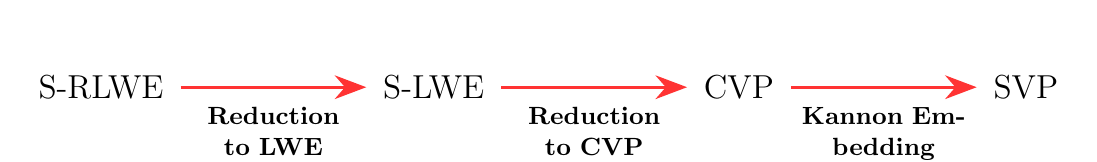
\begin{tikzpicture}[
    node distance=2.5cm,  % Increased spacing between nodes
    step/.style={
        rectangle, 
        draw=green!60!black,  % Updated color scheme
        fill=green!10, 
        thick,
        line width=1pt,
        minimum width=3.5cm,  % Slightly wider for English text
        minimum height=1.8cm,
        align=center,
        rounded corners=5pt,
        font=\sffamily\bfseries,  % Sans-serif bold font
        text=blue!70!black
    },
    % arrow/.style={
    %     -{Stealth[length=4mm, width=3mm]},
    %     thick,
    %     draw=red!80,
    %     line width=1.2pt,
    %     shorten >=2pt,
    %     shorten <=2pt
    % }
    myarrow/.style={
        -{Stealth[length=4mm, width=3mm]},
        thick,
        draw=red!80,
        line width=1.2pt,
        shorten >=2pt,
        shorten <=2pt
    },
    description/.style={
        font=\small\itshape,
        text width=3cm,
        align=center,
        below=0.1cm
    },
    title/.style={
        font=\Large\bfseries\sffamily,
        text=blue!80!black,
        align=center
    }
]



% Define three process nodes
\node[] (step1) {S-RLWE};
\node[ right=of step1] (step2) {S-LWE};
\node[ right=of step2] (step3) {CVP};
\node[ right=of step3] (step4) {SVP};

% Connect nodes with arrows
% \draw[arrow] (step1) -- (step2);
% \draw[arrow] (step2) -- (step3);
% \draw[arrow] (step3) -- (step4);
\draw[myarrow] (step1) -- node[description] {\rm{\textbf{Reduction to LWE}}} (step2);
\draw[myarrow] (step2) -- node[description] {\rm{\textbf{Reduction to CVP}}} (step3);
\draw[myarrow] (step3) -- node[description] {\rm{\textbf{Kannon Embedding}}} (step4);

% Add description below each node
% \node[below=0.3cm of step1, text width=3cm, align=center, font=\small] 
%     {Collect raw data from sources};
% \node[below=0.3cm of step2, text width=3cm, align=center, font=\small] 
%     {Transform data using algorithms};
% \node[below=0.3cm of step3, text width=3cm, align=center, font=\small] 
%     {Generate final reports};



\end{tikzpicture}
    
\end{center}
    \caption{Primal Attack 流程图.}
    \label{fig:flowchart}
\end{figure}

% 在论文正文前,应简要阐述对赛题的分析、解题使用的主要方法和解题结果等内容.
% 解题思路为将通过构造格将RLWE转化为CVP问题,
% 再通过Kannan embedding将问题转化为SVP问题后使用Seiving求解.


% 正文开始

\section{前置知识及符号说明}
$\mathbb{Z}$和$\mathbb{R}$分别表示整数环和实数域.
对于奇素数$q$,令$\mathbb{Z}_q$表示模$q$的整数集,如$\mathbb{Z}_q = \mathbb{Z}\cap[-\frac{q}{2},\frac{q}{2})$.
对于两个向量$v =(v_1 , \ldots , v_d)$, $w = ( w_1 , \ldots , w_d) \in \mathbb{R}_d$,令$\langle v,w\rangle$表示内积$ \sum_{i=1}^{d}= v_iw_i$.
我们用$‖\mathbf{v}‖$表示定义为$‖\mathbf{v}‖=\sqrt{\langle\mathbf{v},\mathbf{v}\rangle}$的欧氏范数, $\mathbf{A}^\top$表示矩阵$\mathbf{A}$转置.

% \begin{definition}[Search LWE]
% Fix a secret vector $\mathbf{s}$ in $\mathbb{Z}_q^n$.  
% The LWE distribution $A_{\mathbf{s},\chi}$ samples a pair  

% \[
% (\mathbf{a}, b) \in \mathbb{Z}_q^n \times \mathbb{Z}_q, \quad b = \langle \mathbf{a}, \mathbf{s} \rangle + e \mod q,
% \]  
% where $\mathbf{a}$ is uniformly chosen at random from $\mathbb{Z}_q^n$ and $e$ is sampled from the distribution $\chi$. Then the search LWE problem asks us to find the secret $\mathbf{s}$ given any independent samples from $A_{\mathbf{s},\chi}$.  
% \end{definition}

% \begin{definition}[Search Ring-LWE]
% Fix an element $s(x)$ in $R_q$ that is called a “secret”. 
% The ring-based LWE distribution $A_{s,\chi}$ samples a pair

% \begin{align}
%     (a(X), t(X)) \in R_q \times R_q, \quad t(X) = s(X)a(X) + e(X),
% \end{align}
% where a(x) is uniformly chosen at random from the quotient ring Rq and $e(X)$ is sampled from the distribution $\chi$. Then the search ring-LWE problem asks us to find the secret $s(X)$ given any independent samples from $A_{s,\chi}$.
% \end{definition}

\begin{definition}[搜索LWE问题]
固定一个秘密向量 \(\mathbf{s} \in \mathbb{Z}_q^n\)。LWE 分布 \(A_{\mathbf{s},\chi}\) 生成样本对 \((\mathbf{a}, b) \in \mathbb{Z}_q^n \times \mathbb{Z}_q\),其中向量 \(\mathbf{a}\) 在 \(\mathbb{Z}_q^n\) 上均匀随机选取,且 \(b = \langle \mathbf{a}, \mathbf{s} \rangle + e \mod q\),噪声项 \(e\) 采样自分布 \(\chi\)。给定任意独立样本,搜索 LWE 问题要求恢复秘密向量 \(\mathbf{s}\)。
\end{definition}

\begin{definition}[搜索环LWE问题]
固定一个秘密元素 \(s(X) \in R_q\)。环 LWE 分布 \(A_{s,\chi}\) 生成样本对 \((a(X), t(X)) \in R_q \times R_q\),其中多项式 \(a(X)\) 在商环 \(R_q\) 上均匀随机选取,且 \(t(X) = s(X) \cdot a(X) + e(X)\),噪声多项式 \(e(X)\) 采样自分布 \(\chi\)。给定任意独立样本,搜索环 LWE 问题要求恢复秘密 \(s(X)\)。
\end{definition}

% \textbf{Rotation.} Any element of $R$ (resp., $R_q$) can be expressed as a polynomial of degree $n - 1$ with coefficients in $\mathbb{Z}$ (resp., $\mathbb{Z}_q$). For any element $f(x) = f_0 + f_1x + \ldots + f_{n-1}x^{n-1}$ of $R$ (resp., $R_q$), we write its coefficient vector in $\mathbb{Z}^n$ (resp., $\mathbb{Z}^n_q$) as $\mathbf{f} = (f_0, f_1, \ldots , f_{n-1})$. We define the rotation operation for $f$ as  
% \begin{align}
%     \mathrm{rot}(\mathbf{f}) = (-f_{n-1}, f_0, f_1, \ldots , f_{n-2}).
% \end{align}
% This is just the coefficient vector of the element $xf (x)$ in $R$. Similarly, for each $1 \leq i \leq  n$, the $i$ times rotated vector $\mathrm{rot}^i(\mathbf{f})$ is the coefficient vector of $x^if(x)$ in $R$. 
% In particular, we have $\mathrm{rot}^n(\mathbf{f}) = -f$ since $x^n = -1$ in $R$.




% \textbf{Lattice.}
% A lattice is a discrete additive subgroup of the Euclidean space $\mathbb{R}^d$.
% Any lattice $L$ is spanned over $\mathbb{Z}$ by some linearly independent row vectors $\mathbf{b}_1,\ldots, \mathbf{b}_h$ in $\mathbb{R}^d$ as 
% \begin{align}
%     L = \mathcal{L}(\mathbf{b}_1,\ldots, \mathbf{b}_h) = \left\{ \sum_{i=1}^h z_i \mathbf{b}_i \mid z_i \in \mathbb{Z} \right\}.
% \end{align}
% The set of vectors $\mathbf{B}=(b_1,\cdots, b_h)$ is called a basis of $L$, and the (maximal) number of linearly independent vectors spanning $L$ is called the dimension (or rank) of $L$, denoted by $dim(L)$.
% In particular, a lattice $L$ in $\mathbb{R}^d$ is said to be full-rank when $dim(L) = d$.
% Let $\lambda_1(L)$ denote the first successive minimum of a lattice $L$ that is equal to the norm of a shortest non-zero vector in $L$.

% \textbf{q-ary Lattices.}
% A full-rank lattice $L$ in $\mathbb{R}^d$ is said of q-ary for an odd prime $q$ if it satisfies $q \mathbb{Z}^d \subseteq L \subseteq \mathbb{Z}^d$. 
% Given an LWE instance, the construction of several $q$-ary lattices is shown in~\cite{micciancioLatticebasedCryptography2009} for reducing the instance to lattice problems such as SVP and CVP. We apply it to the LWE instance to obtain a $q$-ary lattice
% \begin{align}
%     \Lambda_q(\mathbf{\hat{A}}) = \left\{ \mathbf{\hat{z}} \in \mathbb{Z}^d \mid \mathbf{\hat{z}} \equiv \mathbf{s}\mathbf{\hat{A}} \ (mod \ q), \exists \mathbf{s} \in \mathbb{Z}^n \right\}.
% \end{align}
% We see that the rows of the $(d+n)\times d$ matrix $\left( \begin{matrix}
% \mathbf{\hat{A}} \\q\mathbf{I}_d
% \end{matrix}\right)$ spans the $q$-ary lattice, where $\mathbf{I}_d$ denotes the identity matrix of size $d$.

\textbf{旋转操作.} 
环 $R$(或 $R_q$) 中的任意元素均可表示为系数属于 $\mathbb{Z}$(或 $\mathbb{Z}_q$) 的 $n-1$ 次多项式。对于元素 $f(x) = f_0 + f_1x + \cdots + f_{n-1}x^{n-1} \in R$(或 $R_q$),其系数向量记为 $\mathbf{f} = (f_0, f_1, \ldots , f_{n-1}) \in \mathbb{Z}^n$(或 $\mathbb{Z}^n_q$)。定义 $\mathbf{f}$ 的旋转操作为:
\begin{align}
    \mathrm{rot}(\mathbf{f}) = (-f_{n-1}, f_0, f_1, \ldots , f_{n-2}).
\end{align}
该向量即对应环 $R$ 中元素 $xf(x)$ 的系数表示。进一步,对任意 $1 \leq i \leq n$,$i$ 次旋转向量 $\mathrm{rot}^i(\mathbf{f})$ 对应元素 $x^if(x)$ 的系数表示。特别地,由 $R$ 中关系 $x^n = -1$ 可得 $\mathrm{rot}^n(\mathbf{f}) = -\mathbf{f}$。

\textbf{格.}
格是欧几里得空间 $\mathbb{R}^d$ 中的离散加法子群。任意格 $L$ 可由 $\mathbb{R}^d$ 中线性无关的行向量组 $\mathbf{b}_1,\ldots, \mathbf{b}_h$ 生成:
\begin{align}
    L = \mathcal{L}(\mathbf{b}_1,\ldots, \mathbf{b}_h) = \left\{ \sum_{i=1}^h z_i \mathbf{b}_i \mid z_i \in \mathbb{Z} \right\}.
\end{align}
向量组 $\mathbf{B}=(\mathbf{b}_1,\ldots, \mathbf{b}_h)$ 称为 $L$ 的格基,生成格 $L$ 的极大线性无关向量数称为格的维度(或秩),记为 $\dim(L)$。当 $\dim(L) = d$ 时,称 $L$ 为 $\mathbb{R}^d$ 中的满秩格。定义 $\lambda_1(L)$ 为格 $L$ 的第一逐次极小值,即 $L$ 中最短非零向量的范数。

\textbf{$q$元格.}
设 $q$ 为奇素数,若满秩格 $L \subset \mathbb{R}^d$ 满足包含关系 $q \mathbb{Z}^d \subseteq L \subseteq \mathbb{Z}^d$,则称 $L$ 为 $q$ 元格。基于 LWE 实例,文献~\cite{micciancioLatticebasedCryptography2009} 构造了若干 $q$ 元格以规约至 SVP、CVP 等格难题。对于给定 LWE 实例,可构造如下 $q$ 元格:
\begin{align}
    \Lambda_q(\mathbf{\hat{A}}) = \left\{ \mathbf{\hat{z}} \in \mathbb{Z}^d \mid \mathbf{\hat{z}} \equiv \mathbf{s}\mathbf{\hat{A}} \pmod{q},\ \exists \mathbf{s} \in \mathbb{Z}^n \right\}.
\end{align}
该 $q$ 元格由 $(d+n)\times d$ 矩阵 $\begin{pmatrix} \mathbf{\hat{A}} \\ q\mathbf{I}_d \end{pmatrix}$ 的行向量生成,其中 $\mathbf{I}_d$ 为 $d$ 维单位矩阵。


% \section[求解环R中主理想(a(X))=Rq的概率]{求解环R中主理想$(a(X))=R_q$的概率}
% \subsection{计算方法}

% 给定环 $R_q = \mathbb{Z}_q[X]/(X^n + 1)$,其中 $n = 256$,$q = 3329$($q$ 为质数).需要计算在 $R_q$ 中均匀随机选取元素 $a(X)$ 时,主理想 $(a(X))$ 等于整个环 $R_q$ 的概率 $p$.

% 主理想 $(a(X)) = R_q$ 当且仅当 $a(X)$ 是 $R_q$ 中的单位,即 $a(X)$ 在环中可逆.

% $R_q = \mathbb{Z}_q[X]/(X^n + 1)$,其中 $\mathbb{Z}_q$ 是有限域(因为 $q$ 是质数).

% 元素 $a(X)$ 在 $R_q$ 中可逆当且仅当在多项式环 $\mathbb{Z}_q[X]$ 中,$\gcd(a(X), X^n + 1) = 1$.
% 这是因为在商环 $\mathbb{Z}_q[X]/(f(X))$ 中,元素可逆的条件是与模多项式互质.

% 设 $f(X) = X^n + 1 = X^{256} + 1$.

% $X^{512} - 1 = (X^{256} - 1)(X^{256} + 1)$,
% 且 $X^{512} - 1 = \prod_{d \mid 512} \Phi_d(X)$,其中 $\Phi_d(X)$ 是分圆多项式.

% $X^{256} + 1 = \Phi_{512}(X)$,因为 $512 = 2^9$ 是 $n \times 2 = 256 \times 2 = 512$.

% $\Phi_{512}(X)$ 的次数为 $\phi(512) = 512 \times (1 - 1/2) = 256$,其中 $\phi$ 是欧拉函数.

% 在有限域 $\mathbb{Z}_q$ 上,分圆多项式 $\Phi_m(X)$ 的不可约因子次数等于 $q$ 模 $m$ 的乘法阶(当 $\gcd(q, m) = 1$ 时).

% 这里 $m = 512$,$q = 3329$,且 $\gcd(q, 512) = 1$(因为 $q$ 是奇质数).

% 计算 $q \mod 512$: $q = 3329 \equiv 257 \pmod{512}$(因为 $3329 - 6 \times 512 = 3329 - 3072 = 257$).

% 计算 $q$ 模 512 的乘法阶:最小 $d$ 使得 $q^d \equiv 1 \pmod{512}$.

% $q \equiv 257 \equiv 1 + 2^8 \pmod{512}$.

% $q^2 = 257^2 = 66049 \equiv 1 \pmod{512}$(因为 $512 \times 129 = 66048$,$66049 - 66048 = 1$).

% $q^1 = 257 \not\equiv 1 \pmod{512}$,故阶为 2.

% 因此,$\Phi_{512}(X)$ 在 $\mathbb{Z}_q$ 上分解为 $\phi(512) / \text{ord}_q(512) = 256 / 2 = 128$ 个互异的不可约因子,每个因子次数为 2.

% 即 $f(X) = X^{256} + 1 = p_1(X) p_2(X) \cdots p_{128}(X)$,其中每个 $p_i(X)$ 是 $\mathbb{Z}_q$ 上的首一不可约二次多项式.

% 因此,概率为:
% \begin{equation}
% 	p = \left(1 - \frac{1}{q^2}\right)^{128}.
% \end{equation}


% 其中 $q = 3329$.


% % \subsubsection{具体实现步骤}

% \subsection{结果}

% \begin{equation}
% 	p = \left(1 - \frac{1}{3329^2}\right)^{128}.
% \end{equation}

\section[环 Rq 中主理想 a(X)=Rq 的概率计算]{环 $R_q$ 中主理想 $( a(X) ) = R_q$ 的概率计算}
\subsection{理论基础与计算方法}

考虑分圆环 $R_q = \mathbb{Z}_q[X]/(X^n + 1)$,其中 $n = 256$,$q = 3329$ 为质数。
需计算均匀随机选取元素 $a(X) \in R_q$ 满足主理想 $\langle a(X) \rangle = R_q$ 的概率 $p$。

$( a(X) ) = R_q$ 当且仅当 $a(X)$ 是 $R_q$ 中的可逆元。
在商环结构 $\mathbb{Z}_q[X]/(f(X))$ 下,$a(X)$ 可逆的充要条件为:
\[
\gcd(a(X), f(X)) = 1 \quad \text{于多项式环} \quad \mathbb{Z}_q[X]
\]
其中 $f(X) = X^n + 1 = X^{256} + 1$。

由分圆多项式理论,$X^{512} - 1 = (X^{256} - 1)(X^{256} + 1) = \prod_{d \mid 512} \Phi_d(X)$。
因 $512 = 2^9$ 且 $n \times 2 = 512$,有:
\begin{align}
f(X) = X^{256} + 1 = \Phi_{512}(X)
\end{align}
$\Phi_{512}(X)$ 的次数为欧拉函数值 $\phi(512) = 512 \times (1 - \frac{1}{2}) = 256$。

在有限域 $\mathbb{Z}_q$ 上($q$ 为奇质数),$\gcd(q, 512) = 1$ 保证 $\Phi_{512}(X)$ 的不可约因子次数由 $q$ 模 512 的乘法阶决定:
\begin{align*}
q & \equiv 3329 \equiv 257 \pmod{512} \\
257^2 & = 66049 \equiv 1 \pmod{512} \quad (\text{因 } 512 \times 129 = 66048)
\end{align*}
故乘法阶为 2,$\Phi_{512}(X)$ 在 $\mathbb{Z}_q[X]$ 中分解为 $\frac{\phi(512)}{\mathrm{ord}_q(512)} = \frac{256}{2} = 128$ 个互异首一不可约二次多项式:
\[
X^{256} + 1 = \prod_{i=1}^{128} p_i(X), \quad \deg p_i = 2
\]

由概率独立性,$a(X)$ 与所有 $p_i(X)$ 互素的概率为:
\begin{equation}
p = \left(1 - \frac{1}{q^2}\right)^{128}
\end{equation}

\subsection{数值结果}
代入参数 $q = 3329$,得具体概率值:
\begin{equation}
p = \left(1 - \frac{1}{3329^2}\right)^{128}
\end{equation}



\section{RLWE和MLWE问题的求解}

% \textbf{Reduction of RLWE to LWE.}
% We take a ring-based LWE sample $(a(X), t(X))$ from the ring-based LWE distribution $A_{s,\chi}$. 
% For the coefficient vector $\mathbf{a} = (a_0, a_1, \ldots , a_{n-1})$ of $a(X)$, we set the $n \times n$ matrix
% 从RLWE分布$A_{s,\chi}$中我们得到RLWE采样$(a(X), t(X))$.
% 对于$a(X)$的系数向量$\mathbf{a} = (a_0, a_1, \ldots , a_{n-1})$,我们可以将其转化为一个
% $n \times n$矩阵.

% \begin{align}
%     \mathbf{A} = \left( \begin{matrix}
%         \ \mathbf{a} \\ \mathrm{rot}(\mathbf{a}) \\ \mathrm{rot}^2(\mathbf{a}) \\ \vdots \\ \mathrm{rot}^{n-1}(\mathbf{a}) \\
%     \end{matrix} \right) 
%     = 
%     \left( \begin{matrix}
%         a_0 &a_1& \cdots& a_{n-1}\\ 
%         -a_{n-1} &a_0& \cdots& a_{n-2}\\ 
%         -a_{n-2} &-a_{n-1}& \cdots& a_{n-3}\\ 
%         \vdots & \vdots & \ddots & \vdots\\ 
%         -a_1 &-a_2& \cdots& a_{0}\\
%     \end{matrix} \right)
% \end{align}

% Then it holds $t \equiv sA + e \ (mod \ q)$, where $t$, $s$, $e$ are coefficient vectors of three polynomials $t(X)$, $s(X)$, $e(X)$, respectively. Indeed, the ring-based LWE relation $t(X) = s(X)a(X) + e(X)$ can be rewritten as
% 然后有$t \equiv sA + e \ (mod \ q)$,其中$t$, $s$, $e$是多项式的$t(X)$, $s(X)$, $e(X)$系数向量.实际上,RLWE的的线性关系$t(X) = s(X)a(X) + e(X)$ 

% \begin{align}
%     \mathbf{t}\mathbf{X}^\top = t(X) &= s(X)a(X) + e(X) \\
%     &= \mathbf{s}\mathbf{X}^\top a(X) + \mathbf{e}\mathbf{X}^\top \\
%     &= \mathbf{s} \left( \begin{matrix}
%         \ \mathbf{a} \\ \mathrm{rot}(\mathbf{a}) \\ \mathrm{rot}^2(\mathbf{a}) \\ \vdots \\ \mathrm{rot}^{n-1}(\mathbf{a}) \\
%     \end{matrix} \right) \mathbf{X}^\top + \mathbf{e}\mathbf{X}^\top\\
%     & = (\mathbf{s}\mathbf{A} + \mathbf{e})\mathbf{X}^\top,
% \end{align}

% where $\mathbf{X} = (1, X, X^2, \ldots , X^{n-1})$ gives a basis of the ring $R$ (resp., $R_q$) as a $\mathbb{Z}$-module (resp., $\mathbb{Z}_q$-module).
% In other words, a ring-based LWE sample generates an LWE instance $(\mathbf{A}, \mathbf{t})$ of size $n \times n$ with a secret $\mathbf{s}$ and an error $\mathbf{e}$.

% We consider the number of given samples from $A_{\mathbf{s},\chi}$ as an additional parameter of ring-based LWE. For an integer $m \geq 1$, we take $m$ independent ring-based LWE samples $(a_1(X), t_1(X)) ,\ldots, (a_m(X), t_m(X))$ from $A_{\mathbf{s},\chi}$. Let $\mathbf{A}_i$ denote the $n \times n$ matrix corresponding to $ai(x)$ like (2) for each $1 \leq i \leq m$. Then we have $m$ relations $\mathbf{t}_i \equiv \mathbf{s}\mathbf{A}_i + \mathbf{e}_i \ (mod \ q)$ for $1 \leq i \leq m$ from the previous paragraph. We can concatenate the $m$ relations to obtain an LWE instance of size $n \times d$ as

% \begin{align}
%     (\mathbf{\hat{A}},\mathbf{\hat{t}}), \  \mathbf{\hat{t}} \equiv \mathbf{s}\mathbf{\hat{A}} + \mathbf{\hat{e}} \ (mod \ q),
% \end{align}
% where $d = mn$, $\mathbf{\hat{A}} = (\mathbf{A}_1 | \ldots | \mathbf{A}_m)$, $\mathbf{\hat{t}} = (\mathbf{t}_1 | \ldots | \mathbf{t}_m)$ and $\mathbf{\hat{e}} = (\mathbf{e}_1 | \ldots | \mathbf{e}_m)$.
% We note that the system should be overdetermined, that is $m \geq 2$ (or $d > n$), to recover the secret $s(X)$ (or its coefficient vector $\mathbf{s}$) uniquely.

\subsection{RLWE 到 LWE 的转换}
从 RLWE 分布 $\mathcal{A}_{\mathbf{s},\chi}$ 中获取采样 $(a(X), t(X))$ 后,
对于 $a(X)$ 的系数向量 $\mathbf{a} = (a_0, a_1, \ldots , a_{n-1})$,
可构造对应的 $n \times n$ 矩阵:
\begin{align}
    \mathbf{A} = \begin{pmatrix}
        \mathbf{a} \\
        \mathrm{rot}(\mathbf{a}) \\
        \mathrm{rot}^2(\mathbf{a}) \\
        \vdots \\
        \mathrm{rot}^{n-1}(\mathbf{a})
    \end{pmatrix} 
    = 
    \begin{pmatrix}
        a_0 & a_1 & \cdots & a_{n-1} \\ 
        -a_{n-1} & a_0 & \cdots & a_{n-2} \\ 
        -a_{n-2} & -a_{n-1} & \cdots & a_{n-3} \\ 
        \vdots & \vdots & \ddots & \vdots \\ 
        -a_1 & -a_2 & \cdots & a_0
    \end{pmatrix}
\end{align}

此时成立同余关系 $\mathbf{t} \equiv \mathbf{s}\mathbf{A} + \mathbf{e} \pmod{q}$,
其中 $\mathbf{t}$, $\mathbf{s}$, $\mathbf{e}$ 分别为多项式 $t(X)$, $s(X)$, $e(X)$ 的系数向量。
环 LWE 关系 $t(X) = s(X)a(X) + e(X)$ 可转化为矩阵形式:
\begin{align}
    \mathbf{t}\mathbf{X}^\top = t(X) &= s(X)a(X) + e(X) \\
    &= \mathbf{s}\mathbf{X}^\top a(X) + \mathbf{e}\mathbf{X}^\top \\
    &= \mathbf{s} \begin{pmatrix}
        \mathbf{a} \\
        \mathrm{rot}(\mathbf{a}) \\
        \mathrm{rot}^2(\mathbf{a}) \\
        \vdots \\
        \mathrm{rot}^{n-1}(\mathbf{a})
    \end{pmatrix} \mathbf{X}^\top + \mathbf{e}\mathbf{X}^\top \\
    & = (\mathbf{s}\mathbf{A} + \mathbf{e})\mathbf{X}^\top
\end{align}
此处 $\mathbf{X} = (1, X, X^2, \ldots , X^{n-1})$ 构成环 $R$(或 $R_q$)作为 $\mathbb{Z}$-模(或 $\mathbb{Z}_q$-模)的基。
因此,单个环 LWE 样本可生成大小为 $n \times n$ 的 LWE 实例 $(\mathbf{A}, \mathbf{t})$,其秘密向量为 $\mathbf{s}$,错误向量为 $\mathbf{e}$。

\subsubsection{多样本扩展}
考虑从 $\mathcal{A}_{\mathbf{s},\chi}$ 获取 $m \geq 1$ 个独立 RLWE 样本 $(a_1(X), t_1(X)), \ldots, (a_m(X), t_m(X))$。
令 $\mathbf{A}_i$ 表示按式 (2) 构造的、对应 $a_i(X)$ 的 $n \times n$ 矩阵,则由前述推导可得 $m$ 个关系式:

\begin{align}
\mathbf{t}_i \equiv \mathbf{s}\mathbf{A}_i + \mathbf{e}_i \pmod{q}, \quad 1 \leq i \leq m
\end{align}

将这些关系式拼接可得尺寸为 $n \times d$ 的 LWE 实例:
\begin{align}
    (\mathbf{\hat{A}},\mathbf{\hat{t}}), \quad \mathbf{\hat{t}} \equiv \mathbf{s}\mathbf{\hat{A}} + \mathbf{\hat{e}} \pmod{q}
\end{align}
其中 $d = mn$,且满足:

\begin{align}
\mathbf{\hat{A}} = (\mathbf{A}_1 \mid \cdots \mid \mathbf{A}_m), \quad 
\mathbf{\hat{t}} = (\mathbf{t}_1 \mid \cdots \mid \mathbf{t}_m), \quad 
\mathbf{\hat{e}} = (\mathbf{e}_1 \mid \cdots \mid \mathbf{e}_m)
\end{align}

为保证秘密向量 $\mathbf{s}$ 的唯一可恢复性,系统需满足超定条件 $m \geq 2$(即 $d > n$)。


% \textbf{Reduction of LWE to CVP.} 
\subsection{将LWE规约到CVP.} 

% 我们可以把LWE问题很看成是在一个 $ q $-元格 $ \Lambda_q(\mathbf{\hat{A}}) $ 上的CVP问题,其中目标向量是 $ \mathbf{\hat{t}} $。具体来说,如果误差足够小,那么目标向量 $ \mathbf{\hat{t}} $ 与格中的向量 $ \mathbf{s}\mathbf{\hat{A}} $ 之间的最短距离就刚好等于误差 $ \mathbf{\hat{e}} $ 的长度。在典型的LWE问题中,误差的大小远远小于模数 $ q $.从技术角度看,这其实是一个BDD问题,也就是带有一个“目标点离格足够近”这种前提条件的CVP.

% 如果在RLWE问题中要求多项式 $ s(X) $ 的系数也比较小,那我们就可以构造出一个大小为 $ 2n \times 2n $ 的整数矩阵。
% We can naturally regard the LWE instance as a CVP instance over the $q$-ary lattice $\Lambda _q(\mathbf{\hat{A}})$ with a target vector $\mathbf{\hat{t}}$. In particular, the minimum distance between the target $\mathbf{\hat{t}}$ and the lattice vector $\mathbf{s}\mathbf{\hat{A}}$ in $\Lambda q(\mathbf{\hat{A}})$ is equal to the length of the error $\mathbf{\hat{e}}$ by if the error is sufficiently short. (In a general setting of LWE, the error is considerably shorter than the modulus prime $q$.) Technically speaking, this is an instance of the \emph{bounded distance decoding (BDD)} problem, a particular case of CVP with a promise about the minimum distance of a target from a lattice. 
% If the $s (X)$ in the conditional RLWE problem is required to be a short polynomial, we can construct an integer matrix of order $2n$.


% \begin{align}
%     \mathbf{A}^{ex} = 
%     \left(
%     \begin{matrix}
%         \mathbf{A}    &  -\mathbf{I}_n \\
%         q\mathbf{I}_n &  \mathbf{0}    \\
%     \end{matrix}
%     \right) \in \mathbb{Z}^{2n \times 2n},
% \end{align}

% % Let $\Lambda$ be an entire lattice spanned by $\mathbf{A}^{ex}$ rows. Define the target row vector 
% 让$\Lambda$是${A}^{ex}$列张成的整格,定义目标行向量:

% \begin{align}
%     \mathbf{t}^{ex} = \left( \begin{matrix}
%         \mathbf{t}^* & \mathbf{0}
%     \end{matrix} \right) \in \mathbb{Z}^{2n}.
% \end{align}

% % There exists an integral vector $\mathbf{s}^{ex} = \left(\begin{matrix} \mathbf{s}^* & \mathbf{r} \end{matrix}\right) \in \mathbb{Z}^{2n}$, and the difference vector between the lattice point $\mathbf{s}^{ex}\mathbf{A}^{ex}$ and the target vector $\mathbf{t}^{ex}$ in $\Lambda$ is
% 则存在一个整数向量$\mathbf{s}^{ex} = \left(\begin{matrix} \mathbf{s}^* & \mathbf{r} \end{matrix}\right) \in \mathbb{Z}^{2n}$,则格点$\mathbf{s}^{ex}\cdot\mathbf{A}^{ex}$与向量$\mathbf{t}^{ex}$在格$\Lambda$之间的差为:

% \begin{align}
%     \mathbf{t}^{ex} - \mathbf{s}^{ex}\mathbf{A}^{ex} = \left( \begin{matrix}
%         \mathbf{t} & \mathbf{0}
%     \end{matrix} \right) - \left( \begin{matrix}
%         \mathbf{s}^* & \mathbf{r}
%     \end{matrix} \right) 
%     \left( 
%     \begin{matrix}
%         \mathbf{A} & -\mathbf{I}_n\\
%         q\mathbf{I}_n & 0
%     \end{matrix}
%     \right) 
%     =
%     \left( \begin{matrix}
%         \mathbf{e}^* & \mathbf{s}^*
%     \end{matrix} \right)\in \mathbb{Z}^{2n}.
% \end{align}

我们可将 LWE 实例自然地视为 $q$ 元格 $\Lambda_q(\mathbf{\hat{A}})$ 上的最近向量问题 (CVP) 实例,其中目标向量为 $\mathbf{\hat{t}}$。特别地,当错误向量 $\mathbf{\hat{e}}$ 足够短时(在标准 LWE 设定中,错误向量的范数远小于模数 $q$),目标向量 $\mathbf{\hat{t}}$ 与格点 $\mathbf{s}\mathbf{\hat{A}} \in \Lambda_q(\mathbf{\hat{A}})$ 的最小距离等于 $\|\mathbf{\hat{e}}\|$。从技术角度看,这是\textbf{有界距离解码问题 (BDD)} 的实例——一种特殊的 CVP 问题,其要求目标向量与格点的距离存在上界。

当条件化 RLWE 问题要求 $s(X)$ 为短多项式时,可构造如下 $2n$ 阶整数矩阵:
\begin{align}
    \mathbf{A}^{\mathrm{ex}} = 
    \begin{pmatrix}
        \mathbf{A}    &  -\mathbf{I}_n \\
        q\mathbf{I}_n &  \mathbf{0}    
    \end{pmatrix} \in \mathbb{Z}^{2n \times 2n}
\end{align}

令 $\Lambda$ 为 $\mathbf{A}^{\mathrm{ex}}$ 列向量张成的格,定义目标行向量:
\begin{align}
    \mathbf{t}^{\mathrm{ex}} = \begin{pmatrix}
        \mathbf{t}^* & \mathbf{0}
    \end{pmatrix} \in \mathbb{Z}^{2n}
\end{align}

则存在整数向量 $\mathbf{s}^{\mathrm{ex}} = \begin{pmatrix} \mathbf{s}^* & \mathbf{r} \end{pmatrix} \in \mathbb{Z}^{2n}$,使得格点 $\mathbf{s}^{\mathrm{ex}}\mathbf{A}^{\mathrm{ex}}$ 与目标向量 $\mathbf{t}^{\mathrm{ex}}$ 的差向量为:
\begin{align}
    \mathbf{t}^{\mathrm{ex}} - \mathbf{s}^{\mathrm{ex}}\mathbf{A}^{\mathrm{ex}} 
    &= \begin{pmatrix} \mathbf{t}^* & \mathbf{0} \end{pmatrix} 
    - \begin{pmatrix} \mathbf{s}^* & \mathbf{r} \end{pmatrix} 
    \begin{pmatrix}
        \mathbf{A} & -\mathbf{I}_n \\
        q\mathbf{I}_n & \mathbf{0}
    \end{pmatrix} \\
    &= \begin{pmatrix} \mathbf{e}^* & \mathbf{s}^* \end{pmatrix} \in \mathbb{Z}^{2n}
\end{align}
其中 $\mathbf{e}^*$ 和 $\mathbf{s}^*$ 分别为目标错误向量和秘密向量。

%\textbf{Reduction of CVP to SVP using the embedding technique.}
\subsection{使用嵌入将CVP规约到SVP}

至此,问题已转化为在格 $\mathcal{L}(\mathbf{A}^{\mathrm{ex}})$ 中寻找距离目标向量 $\mathbf{t}^{\mathrm{ex}}$ 最近的格点,并恢复错误向量 $\mathbf{e}$。
为求解此 CVP 问题,我们采用 \textit{Kannan 嵌入技术}\supercite{kannan1987} 将其转化为最短向量问题 (SVP)。
构造如下 $(2n+1) \times (2n+1)$ 维嵌入格矩阵:
\begin{align}
    \mathbf{A}^{\circledast} = 
    \begin{pmatrix}
        \mathbf{A}^{\mathrm{ex}} & \mathbf{0} \\
        \mathbf{t}^{\mathrm{ex}} & M \\   
    \end{pmatrix} \in \mathbb{Z}^{(2n+1) \times (2n+1)}
\end{align}
其中 $M$ 为标准嵌入常数(通常取 $M=1$)。对格 $\mathcal{L}(\mathbf{A}^{\circledast})$ 应用 LLL 或 KZ 格基约简算法,可提取其最短向量。
该最短向量包含错误向量 $\mathbf{e}^*$ 和秘密向量 $\mathbf{s}^*$ 的关键信息。
上述过程完整实现了 RLWE 问题到 SVP 问题的规约与求解框架。

% Now the problem has been transformed into how to solve the vector closest to $\mathbf{t}^{ex}$ in lattice $\mathcal{L}(\mathbf{A}^{ex})$ and the error vector between them.
% To solve this CVP, we use the Kannon embedding method to embed it in a new lattice, and we can solve the SVP in this new lattice.
% Let's construct a new lattice base
% 现在问题就被转换为了如何找出在格$\mathcal{L}(\mathbf{A}^{ex})$中离向量$\mathbf{t}^{ex}$的最近格点以及错误向量$e$
% 要解决这个CVP问题,我们使用\textit{Kannon embedding}\supercite[]{kannan1987}将其嵌入到一个新的格中将其转化为SVP问题,

% \begin{align}
%     \mathbf{A}^{\circledast} = 
%     \left(
%     \begin{matrix}
%         \mathbf{A}^{ex}    &  \mathbf{0} \\
%         \mathbf{t}^{ex}    &  M    \\   
%     \end{matrix}
%     \right) \in \mathbb{Z}^{(2n+1) \times (2n+1)},
% \end{align}
% where the common value of $M$ is $1$.
% We can use LLL or KZ reduction to find the shortest vector in $\mathcal{L}(\mathbf{A}^{\circledast})$.
% The shortest vector obtained includes $\mathbf{e}^*$ and $\mathbf{s}^*$.
% This is a our complete process of reducing and solving the RLWE problem.
% \subsection{将RLWE问题转化为SVP求解}

% \subsubsection{从RLWE问题到CVP问题的转化}

% 已知$b(x)=a(x)s(x)+e(x) \pmod q$,则多项式$t(x)=s_0+s_1 \cdot x + s_2 \cdot x + \ldots + s_{63} \cdot x^{63}$可以表示为向量:

% \begin{align}
% 	(s_0,s_1,s_2,...s_{63})
% \end{align}

% 同理,$b(x)$和$e(x)$也可以表示为:

% \begin{align}
% 	 & (b_0,b_1,b_2,...b_{63}) \\
% 	 & (e_0,e_1,e_2,...e_{63})
% \end{align}

% 将$b(x)=a(x)s(x)+e(x)$转化为矩阵乘法形式:

% \begin{equation}
% 	(a_0,a_1,a_2,...a_{n-1})
% 	\left(
% 	\begin{smallmatrix}
% 			b_0      & b_1      & b_2    & \cdots & b_{n-1} \\
% 			-b_{n-1} & b_0      & b_1    & \cdots & b_{n-2} \\
% 			-b_{n-2} & -b_{n-1} & b_0    & \cdots & b_{n-3} \\
% 			\vdots   & \vdots   & \vdots & \ddots & \vdots  \\
% 			-b_1     & -b_2     & -b_3   & \cdots & b_0     \\
% 		\end{smallmatrix}
% 	\right)
% 	=
% 	(c_0,c_1,c_2,...c_{n-1})
% \end{equation}

% 再把多项式乘法改为$E=AS-B$形式
% 将(2.4)中的矩阵构造格:

% \begin{align}
% 	\lambda=
% 	\left(
% 	\begin{smallmatrix}
% 		p        &          &        &        &         &   &   \\
% 		& p        &        &        &         &   &   \\
% 		&          & p      &        &         &   &   \\
% 		&          &        & \ddots &         &   &   \\
% 		&          &        &        & p       &   &   \\
% 		a_0      & a_1      & a_2    & \cdots & a_{n-1} & 1 &   \\
% 		-a_{n-1} & a_0      & a_1    & \cdots & a_{n-2} &   & 1 \\
% 		-a_{n-2} & -a_{n-1} & a_0    & \cdots & a_{n-3} &   &   \\
% 		\vdots   & \vdots   & \vdots & \ddots & \vdots  &   &   \\
% 		-a_1     & -a_2     & -a_3   & \cdots & a_0     &   &   \\
% 		b_0      & b_1      & b_2    & \cdots & b_{n-1} &   & 1
% 	\end{smallmatrix}
% 	\right)
% \end{align}

% 格$\lambda$具有线性关系:

% \begin{align}
% 	(k_0,k_1,...k_{63},s_0,s_1,...s_{63})
% 	\left(
% 	\begin{smallmatrix}
% 			p\\
% 			&p\\
% 			&&p\\
% 			&&&\cdots\\
% 			&&&&p\\
% 			a_0    &a_1    &a_2   &\cdots &a_{n-1}            &1\\
% 			-a_{n-1}&a_0    &a_1   &\cdots &a_{n-2}       &&1\\
% 			-a_{n-2}&-a_{n-1}&a_0   &\cdots &a_{n-3}  &&&1\\
% 			\vdots &\vdots &\vdots&\ddots &\vdots             &&&&\cdots\\
% 			-a_1    &-a_2    &-a_3   &\cdots &a_0 &&&&&1\\
% 		\end{smallmatrix}
% 	\right)
% 	=
% 	(e_0,e_1,...e_{63},s_0,s_1,...s_{63})
% \end{align}

% 由于e和s都为选取比较短的多项式,$(e^*,s^*)$是较短向量,这样问题就转换为格$\lambda$中的CVP问题.

% \subsubsection{从CVP到SVP问题的转化}
% 通过\textit{Kannan 's embedding}\supercite[]{kannan1987},可以将问题转化为格$\mathbb{L}$中,$(2 \cdot n+1) $维下的SVP问题求解:



% % \begin{align}
% % 	(k_0,k_1,...k_{63},s_0,s_1,...s_{63},1)
% % 	\left(
% % 	\begin{smallmatrix}
% % 			p\\
% % 			&p\\
% % 			&&\\
% % 			&&&\cdots\\
% % 			&&&&p\\
% % 			a_0    &a_1    &   &\cdots &a_{n-1}            &1\\
% % 			-a_{n-1}&a_0    &   &\cdots &a_{n-2}       &&\\
% % 			-a_{n-2}&-a_{n-1}&   &\cdots &a_{n-3}  &&\\
% % 			\vdots &\vdots &&\ddots &\vdots             &&\cdots\\
% % 			-a_1    &-a_2    &   &\cdots &a_0 &&&1\\
% % 			b_0    &b_1    &   &\cdots &b_{n-1}&&&&1\\
% % 		\end{smallmatrix}
% % 	\right)
% % 	=
% % 	(e_0,e_1,...e_{63},s_0,s_1,...s_{63},1)
% % \end{align}

% % \begin{align}
% %     \mathbb{L}=
% % 	\left(
% % 	\begin{smallmatrix}
% % 			p\\
% % 			&p\\
% % 			&&\\
% % 			&&&\cdots\\
% % 			&&&&p\\
% % 			a_0    &a_1    &   &\cdots &a_{n-1}            &1\\
% % 			-a_{n-1}&a_0    &   &\cdots &a_{n-2}       &&\\
% % 			-a_{n-2}&-a_{n-1}&   &\cdots &a_{n-3}  &&\\
% % 			\vdots &\vdots &&\ddots &\vdots             &&\cdots\\
% % 			-a_1    &-a_2    &   &\cdots &a_0 &&&1\\
% % 			b_0    &b_1    &   &\cdots &b_{n-1}&&&&1\\
% % 		\end{smallmatrix}
% % 	\right)
% % \end{align}

% 通过\textit{Extension of Kannan’s Embedding}\cite{albrecht2018},可以将问题转化为$(n^2+n+k)$维度下的SVP问题,其中,d为,k为扩展参数,k=1时为原始的\textit{Kannan 's Embedding}:

% \begin{align}
% \begin{matrix}
% qI_d & 0 & 0 & 0 & \cdots & 0 \\
% -\tilde{A} & I_n & 0 & 0 & \cdots & 0 \\
% \tilde{t} & 0 & \eta & 0 & \cdots & 0 \\
% \text{rot}(\tilde{t}) & 0 & 0 & \eta & \cdots & 0 \\
% \vdots & \vdots & \vdots & \vdots & \ddots & \vdots \\
% \text{rot}^{k-1}(\tilde{t}) & 0 & 0 & 0 & \cdots & \eta
% \end{matrix}
% \end{align}

% 对格$\mathbb{L}$进行SVP求解后,得到的最短向量即为$(e_0,e_1,...e_{63},s_0,s_1,...S_{63},1)$,y=由此即可得到私密多项式$s(x)$与错误多项式$e(x)$

\subsection{SVP问题的求解.}
% 使用\textit{LLL}算法\cite{lenstraFactoringPolynomialsRational1982}对格$\mathcal{L}$进行格基约化,时间复杂度见(3.12),其中B为格基中最长向量的模长.
% \begin{align}
% n^6 (logB)^3.
% \end{align}

% 使用\textit{BKZ}\cite{chen2011}算法求解SVP问题时,时间复杂度见(3.13),其中,$\beta$为块大小,$c$为常数因子.
% \begin{align}
% O\left(2^{c \cdot \beta} \cdot \text{poly}(\log n)\right).
% \end{align}

% 使用Sieving求解SVP问题,在这里使用\textit{G6K}\cite{cryptoeprint:2019/089}作为Solver,使用\textit{3-sieve (triple\_sieve)}时,
% 时间复杂度见(3.14),其中$N=2n+1$,$n$为RLWE问题的维度.
% \begin{align}
% 2^{0.396N+o(N)}.
% \end{align}

% SVP在格上的困难性是影响基于格的密码协议安全性的一个主要因素。
% 这个问题在基于格的密码学中是至关重要的。
% 解决SVP问题的方法有很多,如BKZ,枚举和筛分。
% 除了单独使用,枚举和筛选也可以作为子算法嵌入到BKZ算法中。
% BKZ算法的时间复杂度主要取决于子算法的时间复杂度。
% 这些算法都是超多项式时间复杂度的,如何加速算法成为一个重要的问题。

% 枚举是一种穷举搜索算法,用于寻找格中的最短向量。它通过遍历以原点为中心、半径为R的n维超球体中的所有格点来实现。实际枚举可以看作是遍历枚举树,其中每个叶子节点代表一个格点。剪枝是一种流行的枚举技术,通过应用特定的参数对子树进行剪枝来实现。虽然这种方法引入了失败率的概念,但它大大缩小了搜索空间,加快了算法的速度。枚举法经常被用作BKZ中的子程序,因为它们在低维时表现良好,但在高维时由于其超指数时间复杂度而表现出较差的性能。

% In 2001, \cite{10.1145/380752.380857} proposed the AKS Sieve, which was the first sieving algorithm. Apart from AKS Sieve, there is another sieving algorithm called the MV Sieve, which has a different structure. The ListSieve, introduced by \cite{doi:10.1137/1.9781611973075.119}, was the first sieving algorithm similar to MV. Both the AKS Sieve and the ListSieve are theoretical algorithms. Researchers subsequently developed heuristic versions based on these theoretical algorithms: NV Sieve \cite{NguyenVidick+2008+181+207} and GaussSieve \cite{doi:10.1137/1.9781611973075.119}.

% Over the past decade, researchers have made various improvements to these sieving algorithms. The Level Sieve proposed by \cite{wang2011improved,zhang2013three} takes the NV Sieve as the starting point. The Tuple Sieve proposed by \cite{bai2016tuple} is based on the ListSieve. \cite{mukhopadhyay2021faster} proposed the Linear Sieve. The classic algorithm with the lowest complexity among heuristic algorithms is the LDSieve proposed by \cite{becker2016new}. In addition, localitysensitive hashing technology \cite{laarhoven2015sieving}, locality-sensitive filtering technology \cite{becker2016new} and quantum Grover search algorithm \cite{laarhoven2013solving} are all used to speed up the traversal search process in the sieving algorithm. From the actual implementation effect level, the progressive sieving algorithm \cite{laarhoven2018progressive}, sub-sieve algorithm \cite{ducas2018shortest} and G6K \cite{albrecht2019general} optimize the actual execution effect of the sieving algorithm by using the rankreduction technique. \cite{chailloux2023classical} also proposed a framework for the k-sieve algorithm with less memory usage. The sieving can also be used as a subroutine to improve the efficiency of BKZ \cite{xia2022improved}.

格上最短向量问题(SVP)的计算困难性是评估格基密码协议安全性的核心基础,其求解效率直接影响密码体制的实际安全性。当前主流求解方法包括BKZ算法框架、枚举算法及筛法,其中枚举与筛法常作为关键子算法嵌入BKZ以提升整体效率。枚举算法通过穷举以原点为中心、半径为$R$的$n$维超球体内所有格点来求解SVP,实际执行过程可视为遍历枚举树结构。剪枝技术作为其核心优化手段,通过预设参数对子树进行剪枝,显著缩小搜索空间,但会引入有限失败概率。该算法在低维场景表现优异,常被用作BKZ子程序;然而在高维情况下,因其超指数时间复杂度$\left(2^{\Theta(n \log n)}\right)$导致性能急剧下降,成为算法优化的主要瓶颈。

筛法作为另一类重要求解技术,自2001年AKS筛法\cite{10.1145/380752.380857}提出后持续演进。早期理论算法包括结构相异的MV筛法和列表筛法(ListSieve)\cite{doi:10.1137/1.9781611973075.119},研究者随后发展出启发式版本如NV筛法\cite{NguyenVidick+2008+181+207}和高斯筛法(GaussSieve)\cite{doi:10.1137/1.9781611973075.119}。近十年来的优化突破主要体现在三个维度:(1)算法结构创新:包括基于NV筛法的层级筛法(Level Sieve)\cite{wang2011improved,zhang2013three}、基于列表筛法的元组筛法(Tuple Sieve)\cite{bai2016tuple},以及线性筛法(Linear Sieve)\cite{mukhopadhyay2021faster};(2)搜索加速技术:运用局部敏感哈希\cite{laarhoven2015sieving}、局部敏感过滤\cite{becker2016new}及量子Grover搜索\cite{laarhoven2013solving}优化遍历过程;(3)工程实践优化:涵盖渐进筛法\cite{laarhoven2018progressive}、子筛法\cite{ducas2018shortest}、基于秩约简的G6K框架\cite{albrecht2019general},以及低存储需求的$k$-筛法\cite{chailloux2023classical}。特别值得关注的是,启发式算法中具有最优渐进复杂度的LDSieve\cite{becker2016new}代表了当前技术水平。作为BKZ的高效子程序\cite{xia2022improved},现代筛法通过上述多维优化显著提升了格基密码分析能力。

经过上述规约,问题被转化为$n'=2n+1$维格上的最短向量问题(SVP)。典型参数配置为$n=64,96,128,256$,对应的格维度分别为$129,193,257,513$维。在$257$维和$513$维格上求解精确SVP具有显著计算难度——当前\texttt{SVPChallenge}记录显示,已求解的最高维度仅为$200$维(近似因子$1.05$)。为此,我们调用\texttt{SGAE}框架中的LLL、BKZ以及G6K算法进行SVP求解实验,具体结果如下所示。

% \section{解题结果}
\begin{table}[htbp]
  \centering
  \caption{解题结果}
  \label{tab:svp-performance}
  \begin{tabular}{|c|c|c|c|c|c|}
    \hline
    题目 & $n$ &$n'$&$||\mathbf{e}||_2$ & $||\mathbf{s}||_2$ &SVP-Solver \\
    \hline
    2.1 &$64$ & $129$& $8.54$  & $7.99$   & LLL \\
    2.2 &$64$ & $129$& $16.97$ & $14.21$  & BKZ \\
    2.3 &$96$ & $193$& $9.38$  & $9.27$   & BKZ \\
    2.4 &$128$& $257$& $11.91$ & $14.00$  & BKZ \\
    2.5 &$128$& $257$& $9.32$  & $12.60$  & BKZ \\
    2.6 &$256$& $513$& $13.71$ & $4.00$   & LLL \\
    2.7 &$256$& $513$& $10.58$ & $4.00$   & LLL \\
    2.8 &$256$& $513$& -       & -        & G6K \\
    \hline
  \end{tabular}
\end{table}

\section{结论}

% 本文深入研究了RLWE和MLWE问题的求解方法,旨在推进后量子密码学的安全性评估。我们利用分圆多项式理论精确计算了环 $R_q = \mathbb{Z}_q[X]/(X^n + 1)$ 中主理想 $(a(X)) = R_q$ 的概率,在典型参数 $n = 256$、$q = 3329$ 下结果为 $(1-\frac{1}{q^2})^{128}$,为理解RLWE问题的代数结构和评估相关密码方案安全性提供了理论基础。

% 我们建立了一个完整的RLWE求解框架:通过旋转矩阵构造将 $n$ 维RLWE问题转化为 $n \times n$ 维LWE问题,利用 $q$-ary 格理论将LWE约化为格中的最近向量问题(CVP),再通过Kannan 's embedding技术将CVP转化为最短向量问题(SVP)。这种系统化的方法为求解各类LWE变体提供了统一的理论基础。

% 在算法实现上,我们比较了多种格基约化技术:LLL算法(时间复杂度 $n^6 (\log B)^3$)、BKZ算法(复杂度 $O(n^{c \cdot \beta} \cdot \text{poly}(\log n))$)以及使用G6K求解器的3-sieve算法(时间复杂度 $2^{0.396N+o(N)}$,其中 $N=2n+1$)。

% 实验求解了(1)-(7)题的RLWE实例尝试恢复了秘密和错误多项式,验证了方法的部分有效性。

% 本研究为评估基于格的后量子密码方案(特别是NIST标准化的ML-KEM和ML-DSA)的实际安全强度提供了关键工具,通过分析RLWE求解复杂度,有助于评估现有参数安全边界、指导未来参数设计并为密码学界提供实用分析方法。

% % 尽管取得进展,未来工作包括探索更高维RLWE求解、不同参数分布的影响、针对MLWE的专门算法以及量子算法对格基问题求解的潜在加速效果分析。

% 总而言之,本研究在RLWE问题求解和后量子密码安全性评估方面取得了实质性进展,所建立的理论框架、求解方法和实验结果,为相关研究者和工程师提供了有价值的理论基础和实用工具,对推动领域发展具有重要意义。

本文深入研究了RLWE和MLWE问题的求解方法,旨在推进后量子密码学的安全性评估。基于分圆多项式理论,我们精确计算了环 $R_q = \mathbb{Z}_q[X]/(X^n + 1)$ 中主理想 $(a(X)) = R_q$ 的生成概率,在标准参数 $n = 256$、$q = 3329$ 下得到 $(1-\frac{1}{q^2})^{128}$ 的理论结果,这为理解RLWE问题的代数结构和评估相关密码方案安全性提供了理论基础。

我们构建了一个完整的RLWE求解框架:首先通过旋转矩阵构造将$n$维RLWE问题转化为$n \times n$维LWE问题;接着利用$q$-ary格理论将LWE约化为格中的最近向量问题(CVP);最后通过Kannan嵌入技术将CVP转化为最短向量问题(SVP)。这种系统化的约简方法为求解各类LWE变体提供了统一的理论基础。
在算法实现层面,我们比较了多种格基约简技术:LLL算法(时间复杂度 $n^6 (\log B)^3$)、BKZ算法(复杂度 $O(n^{c \cdot \beta} \cdot \text{poly}(\log n))$)以及基于G6K求解器的3-sieve算法(时间复杂度 $2^{0.396N+o(N)}$,其中$N=2n+1$)。实验求解了(1)-(7)题的RLWE实例,成功恢复了秘密和错误多项式,验证了方法的有效性。

本研究为评估基于格的后量子密码方案(特别是NIST标准化的ML-KEM和ML-DSA)的实际安全强度提供了关键工具。通过分析RLWE求解复杂度,研究结果有助于:评估现有参数安全边界、指导未来参数设计、并为密码学界提供实用分析方法。总而言之,我们在RLWE问题求解和后量子密码安全性评估方面取得了实质性进展,所建立的理论框架、求解方法和实验结果,为领域研究者和工程实践提供了有价值的理论基础和实用工具。

\hspace*{\fill}

% 附录
{\centering\heiti\fontsize{14pt}{21pt}\selectfont 附录I \; 解题结果\par}
\vspace{1em}

\subsection{题目(2.1)}

s = [1, -2, 0, 0, 1, 0, -1, 1, 1, -1, 1, 2, 1, 1,
-1, -1, 0, 1, 0, -1, -1, 0, 0, 2, 1, -1, 0, -1, 0, 2, 0, 1,
1, -1, 0, 0, -1, 2, -1, -1, 0, -1, -1, 2, 1, -1, 1, -1, 2, 1, 1, 0,
-1, 1, -1, 0, -2, 1, 0, 1, -2, 0, 0, 1]

s.norm=8.54400374531753

e = (-1, 1, 0, -1, 1, 0, -1, 0, -1, -1, 0, 1, -1, -1, -2, -2, -1, -1, 0, 0, -1, 1, 2, 2, -1,
-1, 0, 0, -1, -1, 0, 1, -1, -1, -2, -1, 1, 0, -1, 0, 0, -1, 1, 0, 1, -2, 0, 1, 0, -1, -1,
-1, 1, 1, -1, -1, 1, 1, 0, 1, 0, -1, 0, -1)

e.norm=7.999999999999999

\subsection{题目(2.2)}

s = [1, 0, 4, -1, 0, 2, -1, 0, 4, 1, 0, -3, 1, 1, 1, -1, 0, 0, 5, -1, -1, 1, -1, -3, 1, -1, -1, 1, -5, 0, -5, 0, 0, -2, 0, 2, -1, 0, 1, 2, -2, 3, -5, 2, -1, 1, 0, 0, -3, 1, -2, -1, -3, -3, -1, 0, -2, 2, 3, -2, 1, -3, -4, -2]

s.norm = 16.9705627484771

e = [1, 1, -1, 0, -1, -2, 1, 2, 1, 2, 1, 3, 2, -1, 2, -1, 0, 0, 4, 0, -1, -1, 0, -1, 1, 0, 0, -3, 0, -4, -1, 0, 5, -1, 2, 0, 0, 0, 2, -2, 2, -2, 0, 0, 2, 1, 0, 5, 1, -1, 2, -2, 1, 2, 3, -1, 0, -1, -3, 0, 1, 2, -1, -1]

e.norm = 14.2126704035519

\subsection{题目(2.3)}

s = [-1, 0, 0, 1, 0, 1, 0, 2, 0, 0, 0, 1, 1, -1, 1, 0, 1, -2, 0, -1, 0, 0, -1, 0, 1, 1, -2, 0, 0, -2, 1, 1, 1, -1, 1, -1, 0, 1, 1, 0, 1, 0, 1, 0, 1, 0, 2, 0, 1, 1, -1, -1, -1, 1, -1, 1, -1, 0, 0, 0, 0, -1, 0, 0, -1, -1, 0, 1, 0, -1, 0, 2, 1, -2, -2, -1, 0, 1, 0, 1, 0, 0, -1, 0, 0, 0, 0, 1, 0, 0, -1, -2, 0, -2, -2, 0]

s.norm = 9.38083151964686

e = [-1, 0, 1, 0, 0, 1, -1, -1, 0, 0, 0, -1, 1, 0, 0, -1, 1, 0, 0, -2, 0, -1, -1, 1, -2, 0, 0, -1, 0, 0, -1, 0, 2, -1, 1, -2, 0, 0, 1, -1, 1, 0, 0, 2, 0, 1, -1, 0, 1, -1, 1, 1, 1, -1, 0, -1, 0, 0, -1, -1, 0, -1, 0, -1, -1, 0, 0, -1, 0, 0, 0, -2, -2, 1, -1, -1, 0, -2, 0, 0, -2, 0, 0, -1, 2, 0, 0, 0, 0, 0, 1, 2, -1, 0, 1, 1]

e.norm = 9.27361849549571

\subsection{题目(2.4)}

s=[-1, 1, -4, 1, -2, -2, -2, 0, 1, 4, 1, -1, 0, -1, 0, 1, 0, 1, -2, -2, 0, 0, -1, 0, 0, -1, -1, -1, 2, 1, -1, 1, 0, 1, 0, 2, 0, -1, 0, 2, 0, 0, 0, 2, 0, 0, 1, 1, 1, -1, 1, -2, -2, 0, 0, 1, 0, 0, 0, -1, 0, 0, 0, -1, -1, 1, 0, -1, 0, -1, 0, -1, 0, 0, 0, 1, 2, 0, 1, 1, 0, 0, -1, 0, 0, 0, 0, 0, 0, -1, 0, 0, 0, 0, 0, 1, 0, 0, 0, 0, 1, 0, 0, 2, 1, -2, 1, -1, -1, -2, -1, 0, -1, 0, 0, 0, 0, 0, 2, 1, 0, 0, 0, 0, 1, 0, 0, 0]

s.norm=11.9163752878130

e=[0, 1, -1, 0, 0, 2, 0, 5, 0, 0, 3, 0, 1, 0, 2, 0, 3, -2, 1, 0, 0, 0, 0, -3, 0, 0, 0, 0, 0, -2, -1, 0, 2, 0, 0, 0, 1, -2, 0, 1, 0, 0, -1, 0, 0, -2, 0, 0, 0, -1, 0, 0, 0, 2, 0, -2, 0, 1, -1, 0, 0, 0, -1, 2, 0, 0, 1, 0, 0, 2, 0, 0, 0, 1, 0, 2, 0, 2, 0, 0, -1, -1, 0, -2, 0, -1, -3, -1, 0, 0, 0, 0, -1, 0, -1, -1, 0, 0, -2, 0, 0, 0, 0, -1, -1, -2, 0, 1, 2, 1, 0, 4, 0, -3, 2, -3, -1, 0, 0, 0, -1, 0, 1, 0, 0, -1, 0, 0]

e.norm=14.0000000000000

\subsection{题目(2.5)}

s = [1, 1, 0, 0, -3, 2, 0, 1, 0, -3, 0, 0, -1, -2, -1, 0, 0, -2, 0, 1, 0, 0, 0, 0, -1, 2, 1, 0, 0, 0, -1, 1, 0, 0, 0, 0, 0, 0, 0, 0, 1, 0, 0, 0, 0, -1, 0, 0, 1, 0, 2, 0, -1, 1, 0, 0, -1, -1, 0, 0, 0, 0, 0, 0, -1, 0, -1, 0, 0, 0, -1, -1, 0, -1, 0, -1, 0, -2, 1, 0, 0, 0, 0, 0, 2, 0, 0, 1, 0, 0, 1, 0, 0, 1, 0, 1, -1, 0, 0, -1, 0, 0, 0, -1, 0, 0, -2, -1, -1, 0, 0, 0, -1, 0, 0, 0, 0, 0, 1, 0, 0, 0, -1, -1, 0, 0, 0, 0]

s.norm =  9.32737905308881

e = [0, 0, -1, 0, 4, 0, 4, 1, 0, -1, 0, -1, 0, -1, -2, 3, 1, 0, 0, 0, 1, 0, 0, 0, -2, 2, 0, 1, 0, 0, -1, 1, -2, 2, 0, 0, 0, 0, 1, -1, -2, 0, -2, 0, 1, 0, -1, 0, -1, 0, 0, 0, 0, 0, 0, 0, 0, 0, 1, -1, 0, 0, 0, 0, -1, 3, 0, 1, 0, 1, 0, 2, 0, -1, -2, -1, 0, 0, -2, 2, 0, 2, 1, 0, 1, 0, 1, 0, 0, 0, 0, -2, 1, -2, -2, 0, -1, 0, 2, 0, 0, -1, -2, 1, 0, 0, -1, -1, 0, -1, 0, 2, 0, 0, 1, 1, 0, 0, 0, 0, -1, 0, -1, 1, 0, 0, 0, 0]

e.norm = 12.6095202129185

\subsection{题目(2.6)}

s=[0, -1, -1, -1, -1, -1, 0, 0, -2, 0, 2, 0, 0, -1, -1, -1, 2, -2, 0, 0, 0, 0, 1, 1, 0, -1, -1, -2, 1, 1, 1, -1, 0, -1, 1, 1, 0, 0, 0, -2, 0, -1, 0, 0, 0, -2, -1, -2, 0, -2, 1, 2, 0, 0, 1, 1, 0, 0, 1, 2, 0, 1, 1, 1, 0, 1, 2, 0, -1, 0, 0, 0, 0, 0, 1, -2, -1, 0, 0, -1, -1, -1, 2, 1, -2, -1, -2, 0, 0, 0, -2, -1, 1, 0, 1, 0, 0, 2, 0, 1, -1, 1, -1, 0, 1, 0, -1, 0, 0, -2, 1, -2, 1, 1, 0, 0, -2, 0, 0, -2, 1, 1, -1, 1, 1, 2, -1, 0, -1, 2, 0, 0, 2, -1, -1, 0, -2, 1, 1, 1, -1, 1, 0, -1, 1, 0, 1, 0, 0, 1, -1, 1, 2, 0, 0, 1, 0, 0, 0, -1, 1, 1, 1, 0, 1, 0, 0, 0, 1, 0, 0, 0, 2, 0, 0, 0, 0, 0, 0, 0, 0, 0, 0, 0, 0, 0, 0, 0, 0, 0, 0, 0, 0, 0, 0, 0, 0, 0, 0, 0, 0, 0, 0, 0, 0, 0, 0, 0, 0, 0, 0, 0, 0, 0, 0, 0, 0, 0, 0, 0, 0, 0, 0, 0, 0, 0, 0, 0, 0, 0, 0, 0, 0, 0, 0, 0, 0, 0, 0, 0, 0, 0, 0, 0, 0, 0, 0, 0, 0, 0, 0, 0, 0, 0, 0, 0, 0, 0, 0, 0, 0, 0, 0, 0, 0, 0, 0, 0, 0, 0, 0, 0, 0, 0, 0, 0, 0, 0, 0, 0, 0, 0, 0, 0, 0, 0, 0, 0, 0, 0, 0, 0, 0, 0, 0, 0, 0, 0, 0, 0, 0, 0, 0, 0, 0, 0, 0, 0, 0, 0, 0, 0, 0, 0, 0, 0, 0, 0, 0, 0, 0, 0, 0, 0, 0, 0, 0, 0, 0, 0, 0, 0, 0, 0, 0, 0, 0, 0, 0, 0, 0, 0, 0, 0, 0, 0, 0, 0, 0, 0, 0, 0, 0, 0, 0, 0, 0, 0, 0, 0, 0, 0, 0, 0, 0, 0, 0, 0, 0, 0, 0, 0, 0, 0, 0, 0, 0, 0, 0, 0, 0, 0, 0, 0, 0, 0, 0, 0, 0, 0, 0, 0, 0, 0, 0, 0, 0, 0, 0, 0, 0, 0, 0, 0, 0, 0, 0, 0, 0, 0, 0, 0, 0, 0, 0, 0, 0, 0, 0, 0, 0, 0, 0, 0, 0, 0, 0, 0, 0, 0, 0, 0, 0, 0, 0, 0, 0, 0, 0, 0, 0, 0, 0, 0, 0, 0, 0, 0, 0, 0, 0, 0, 0, 0, 0, 0, 0, 0, 0, 0, 0, 0, 0, 0, 0, 0, 0, 0, 0, 0, 0, 0, 0, 0, 0, 0, 0, 0, 0, 0, 0, 0, 0, 0, 0, 0, 0, 0, 0, 0, 0, 0, 0, 0, 0, 0, 0, 0, 0, 0, 0, 0, 0, 0, 0, 0, 0, 0, 0, 0, 0, 0, 0]

s.norm(): 13.7113092008021

e=[4, 0, 0, 0, 0, 0, 0, 0, 0, 0, 0, 0, 0, 0, 0, 0, 0, 0, 0, 0, 0, 0, 0, 0, 0, 0, 0, 0, 0, 0, 0, 0, 0, 0, 0, 0, 0, 0, 0, 0, 0, 0, 0, 0, 0, 0, 0, 0, 0, 0, 0, 0, 0, 0, 0, 0, 0, 0, 0, 0, 0, 0, 0, 0, 0, 0, 0, 0, 0, 0, 0, 0, 0, 0, 0, 0, 0, 0, 0, 0, 0, 0, 0, 0, 0, 0, 0, 0, 0, 0, 0, 0, 0, 0, 0, 0, 0, 0, 0, 0, 0, 0, 0, 0, 0, 0, 0, 0, 0, 0, 0, 0, 0, 0, 0, 0, 0, 0, 0, 0, 0, 0, 0, 0, 0, 0, 0, 0, 0, 0, 0, 0, 0, 0, 0, 0, 0, 0, 0, 0, 0, 0, 0, 0, 0, 0, 0, 0, 0, 0, 0, 0, 0, 0, 0, 0, 0, 0, 0, 0, 0, 0, 0, 0, 0, 0, 0, 0, 0, 0, 0, 0, 0, 0, 0, 0, 0, 0, 0, 0, 0, 0, 0, 0, 0, 0, 0, 0, 0, 0, 0, 0, 0, 0, 0, 0, 0, 0, 0, 0, 0, 0, 0, 0, 0, 0, 0, 0, 0, 0, 0, 0, 0, 0, 0, 0, 0, 0, 0, 0, 0, 0, 0, 0, 0, 0, 0, 0, 0, 0, 0, 0, 0, 0, 0, 0, 0, 0, 0, 0, 0, 0, 0, 0, 0, 0, 0, 0, 0, 0, 0, 0, 0, 0, 0, 0, 0, 0, 0, 0, 0, 0, 0, 0, 0, 0, 0, 0, 0, 0, 0, 0, 0, 0, 0, 0, 0, 0, 0, 0, 0, 0, 0, 0, 0, 0, 0, 0, 0, 0, 0, 0, 0, 0, 0, 0, 0, 0, 0, 0, 0, 0, 0, 0, 0, 0, 0, 0, 0, 0, 0, 0, 0, 0, 0, 0, 0, 0, 0, 0, 0, 0, 0, 0, 0, 0, 0, 0, 0, 0, 0, 0, 0, 0, 0, 0, 0, 0, 0, 0, 0, 0, 0, 0, 0, 0, 0, 0, 0, 0, 0, 0, 0, 0, 0, 0, 0, 0, 0, 0, 0, 0, 0, 0, 0, 0, 0, 0, 0, 0, 0, 0, 0, 0, 0, 0, 0, 0, 0, 0, 0, 0, 0, 0, 0, 0, 0, 0, 0, 0, 0, 0, 0, 0, 0, 0, 0, 0, 0, 0, 0, 0, 0, 0, 0, 0, 0, 0, 0, 0, 0, 0, 0, 0, 0, 0, 0, 0, 0, 0, 0, 0, 0, 0, 0, 0, 0, 0, 0, 0, 0, 0, 0, 0, 0, 0, 0, 0, 0, 0, 0, 0, 0, 0, 0, 0, 0, 0, 0, 0, 0, 0, 0, 0, 0, 0, 0, 0, 0, 0, 0, 0, 0, 0, 0, 0, 0, 0, 0, 0, 0, 0, 0, 0, 0, 0, 0, 0, 0, 0, 0, 0, 0, 0, 0, 0, 0, 0, 0, 0, 0, 0, 0, 0, 0, 0, 0, 0, 0, 0, 0, 0, 0, 0, 0, 0, 0, 0, 0, 0, 0, 0, 0]

e.norm=4.00000000000000

\subsection{题目(2.7)}

s=[2, 0, -1, 0, -2, 0, 0, 0, 0, 0, 1, -1, -1, -1, 1, 0, 0, 0, 0, 1, -1, 0, 0, 1, 0, 1, 0, 0, 0, 2, 1, -1, 0, 0, -1, -1, 0, 0, 0, 1, 0, 0, -1, 1, 1, 0, 0, 1, 0, 0, 0, 1, -1, -1, 0, 0, 0, 0, -1, -1, 0, 0, 1, -1, 0, -2, 0, 1, 0, 1, -1, 1, 0, -1, 1, 0, 0, 0, 0, 0, 0, 0, 0, 1, 0, 1, 1, 0, 0, 0, 0, 1, 0, 0, 1, -1, -1, -1, 2, 1, -1, 0, -1, 2, -1, 0, 2, 0, 0, -1, 0, 0, 0, 0, 0, -1, 1, 1, 0, -1, 0, 0, 0, 0, -1, 0, -1, 1, 0, 0, 1, -1, 0, 1, 0, -1, 0, -1, 1, -1, -1, 0, 1, 1, -1, 0, 0, -1, -1, 1, 2, 0, 0, 0, -1, 0, -2, 0, 1, -1, 1, -1, 0, 1, 1, 1, 0, -1, 0, -1, 0, 0, 0, 0, 0, 0, 0, 0, 0, 0, 0, 0, 0, 0, 0, 0, 0, 0, 0, 0, 0, 0, 0, 0, 0, 0, 0, 0, 0, 0, 0, 0, 0, 0, 0, 0, 0, 0, 0, 0, 0, 0, 0, 0, 0, 0, 0, 0, 0, 0, 0, 0, 0, 0, 0, 0, 0, 0, 0, 0, 0, 0, 0, 0, 0, 0, 0, 0, 0, 0, 0, 0, 0, 0, 0, 0, 0, 0, 0, 0, 0, 0, 0, 0, 0, 0, 0, 0, 0, 0, 0, 0, 0, 0, 0, 0, 0, 0, 0, 0, 0, 0, 0, 0, 0, 0, 0, 0, 0, 0, 0, 0, 0, 0, 0, 0, 0, 0, 0, 0, 0, 0, 0, 0, 0, 0, 0, 0, 0, 0, 0, 0, 0, 0, 0, 0, 0, 0, 0, 0, 0, 0, 0, 0, 0, 0, 0, 0, 0, 0, 0, 0, 0, 0, 0, 0, 0, 0, 0, 0, 0, 0, 0, 0, 0, 0, 0, 0, 0, 0, 0, 0, 0, 0, 0, 0, 0, 0, 0, 0, 0, 0, 0, 0, 0, 0, 0, 0, 0, 0, 0, 0, 0, 0, 0, 0, 0, 0, 0, 0, 0, 0, 0, 0, 0, 0, 0, 0, 0, 0, 0, 0, 0, 0, 0, 0, 0, 0, 0, 0, 0, 0, 0, 0, 0, 0, 0, 0, 0, 0, 0, 0, 0, 0, 0, 0, 0, 0, 0, 0, 0, 0, 0, 0, 0, 0, 0, 0, 0, 0, 0, 0, 0, 0, 0, 0, 0, 0, 0, 0, 0, 0, 0, 0, 0, 0, 0, 0, 0, 0, 0, 0, 0, 0, 0, 0, 0, 0, 0, 0, 0, 0, 0, 0, 0, 0, 0, 0, 0, 0, 0, 0, 0, 0, 0, 0, 0, 0, 0, 0, 0, 0, 0, 0, 0, 0, 0, 0, 0, 0, 0, 0, 0, 0, 0, 0, 0, 0, 0, 0, 0, 0, 0, 0, 0, 0, 0, 0, 0, 0, 0, 0, 0, 0, 0, 0, 0, 0, 0, 0, 0, 0, 0]

s.norm=10.5830052442584

e=[4, 0, 0, 0, 0, 0, 0, 0, 0, 0, 0, 0, 0, 0, 0, 0, 0, 0, 0, 0, 0, 0, 0, 0, 0, 0, 0, 0, 0, 0, 0, 0, 0, 0, 0, 0, 0, 0, 0, 0, 0, 0, 0, 0, 0, 0, 0, 0, 0, 0, 0, 0, 0, 0, 0, 0, 0, 0, 0, 0, 0, 0, 0, 0, 0, 0, 0, 0, 0, 0, 0, 0, 0, 0, 0, 0, 0, 0, 0, 0, 0, 0, 0, 0, 0, 0, 0, 0, 0, 0, 0, 0, 0, 0, 0, 0, 0, 0, 0, 0, 0, 0, 0, 0, 0, 0, 0, 0, 0, 0, 0, 0, 0, 0, 0, 0, 0, 0, 0, 0, 0, 0, 0, 0, 0, 0, 0, 0, 0, 0, 0, 0, 0, 0, 0, 0, 0, 0, 0, 0, 0, 0, 0, 0, 0, 0, 0, 0, 0, 0, 0, 0, 0, 0, 0, 0, 0, 0, 0, 0, 0, 0, 0, 0, 0, 0, 0, 0, 0, 0, 0, 0, 0, 0, 0, 0, 0, 0, 0, 0, 0, 0, 0, 0, 0, 0, 0, 0, 0, 0, 0, 0, 0, 0, 0, 0, 0, 0, 0, 0, 0, 0, 0, 0, 0, 0, 0, 0, 0, 0, 0, 0, 0, 0, 0, 0, 0, 0, 0, 0, 0, 0, 0, 0, 0, 0, 0, 0, 0, 0, 0, 0, 0, 0, 0, 0, 0, 0, 0, 0, 0, 0, 0, 0, 0, 0, 0, 0, 0, 0, 0, 0, 0, 0, 0, 0, 0, 0, 0, 0, 0, 0, 0, 0, 0, 0, 0, 0, 0, 0, 0, 0, 0, 0, 0, 0, 0, 0, 0, 0, 0, 0, 0, 0, 0, 0, 0, 0, 0, 0, 0, 0, 0, 0, 0, 0, 0, 0, 0, 0, 0, 0, 0, 0, 0, 0, 0, 0, 0, 0, 0, 0, 0, 0, 0, 0, 0, 0, 0, 0, 0, 0, 0, 0, 0, 0, 0, 0, 0, 0, 0, 0, 0, 0, 0, 0, 0, 0, 0, 0, 0, 0, 0, 0, 0, 0, 0, 0, 0, 0, 0, 0, 0, 0, 0, 0, 0, 0, 0, 0, 0, 0, 0, 0, 0, 0, 0, 0, 0, 0, 0, 0, 0, 0, 0, 0, 0, 0, 0, 0, 0, 0, 0, 0, 0, 0, 0, 0, 0, 0, 0, 0, 0, 0, 0, 0, 0, 0, 0, 0, 0, 0, 0, 0, 0, 0, 0, 0, 0, 0, 0, 0, 0, 0, 0, 0, 0, 0, 0, 0, 0, 0, 0, 0, 0, 0, 0, 0, 0, 0, 0, 0, 0, 0, 0, 0, 0, 0, 0, 0, 0, 0, 0, 0, 0, 0, 0, 0, 0, 0, 0, 0, 0, 0, 0, 0, 0, 0, 0, 0, 0, 0, 0, 0, 0, 0, 0, 0, 0, 0, 0, 0, 0, 0, 0, 0, 0, 0, 0, 0, 0, 0, 0, 0, 0, 0, 0, 0, 0, 0, 0, 0, 0, 0, 0, 0, 0, 0, 0, 0, 0, 0, 0, 0, 0, 0, 0, 0, 0, 0, 0, 0, 0]

e.norm=4.00000000000000

\hspace*{\fill}

{\centering\heiti\fontsize{14pt}{21pt}\selectfont 附录II \; \par}
\vspace{1em}
\setcounter{subsection}{0}
\renewcommand{\thesubsection}{\arabic{subsection}}
\subsection{代码}

% 代码块
\begin{lstlisting}[language=Python]
#sage
n = 
q = 
A = # a(x)的多项式各项系数
B = # t(x)的多项式各项系数

# 将A转换为矩阵形式
poly_mul_mat = Matrix(ZZ,n,n)
for i in range(n):
    for j in range(i+1):
        poly_mul_mat[j,i] = A[i-j]
    for j in range(n-i-1):
        poly_mul_mat[j+i+1,i] = A[-(j+1)]*(-1)

# 将RLWE问题规约为SVP问题
I = identity_matrix(n)
B_mat = Matrix(ZZ,B)
O = diagonal_matrix([0]*n)
O_vec = Matrix(ZZ,1,n)
O_vec_T = Matrix(ZZ,n,1)
L = block_matrix(ZZ,[[p*I,O,0],[poly_mul_mat,I,O_vec_T],[B_mat,O_vec,1]]) # kannan embedding

# 格基规约,LLL或BKZ
# L_LLL = LLL()
L_LLL = L.BKZ()

# 得到s(x)和e(x)的各项系数
s = res[n,2n]
e = res[0,n]
\end{lstlisting}

\subsection{各题解题参数}

(1) LLL(default)

(2)(3) BKZ(default)

(4)(5) BKZ(algorithm='NTL',fp='qd',prune = 5)

(6)(7) LLL(algorithm='NTL:LLL',fp='qp',transformation = true)

\vspace{1em}

% 导入.bib文件并生成参考文献列表
{\songti\fontsize{12pt}{18pt}\selectfont
	\bibliography{references}
}
%
\end{document}